% *******************************************************************************
% * Copyright (c) 2007 by Elexis
% * All rights reserved. This document and the accompanying materials
% * are made available under the terms of the Eclipse Public License v1.0
% * which accompanies this distribution, and is available at
% * http://www.eclipse.org/legal/epl-v10.html
% *
% *  $Id: omnivore.tex 2933 2007-07-29 10:05:35Z rgw_ch $
% *******************************************************************************
% !Mode:: "TeX:UTF-8" (encoding info for WinEdt)

\section{Elexis-Omnivore}
Ein \textit{Allesfresser-Plugin}, das Dokumente aller Art einem Patienten zuordnen kann. Dieses Plugin bietet, nebst der Methode mit \href{http://www.elexis.ch/jp/index.php?option=content&task=view&id=107}{OpenOffice}, eine zweite Möglichkeit der Dokumentenverwaltung mit Elexis.

\begin{wrapfigure}{l}{7cm}
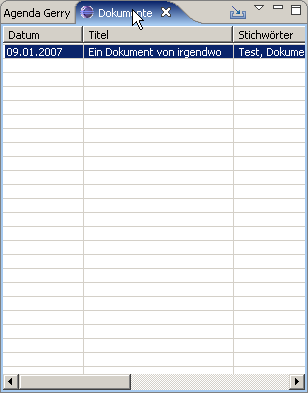
\includegraphics[width=7cm]{images/omnivore1}
% omnivore1.png: 308x393 pixel, 96dpi, 8.15x10.40 cm, bb=0 0 231 295
\end{wrapfigure}

Die Methode mit Omnivore hat den Vorteil, dass alle Dokumente in ihrem Originalformat bleiben. Dies hat aber auch den Nachteil, dass die Dokumente nur mit den dazugehörigen Programmen wieder gelesen werden können. Wenn Sie beispielsweise Dokumente im PDF-Format  hier abspeichern, dann müssen Sie zum Lesen auch den Acrobat Reader oder ein dazu kompatibles Programm haben. Wenn Sie dies beachten, dann ist die Arbeit mit Omnivore sehr einfach:\\
\medskip
Öffnen Sie die View Omnivore-Dokumente:
Sie finden eine Tabelle mit allen Dokumenten, welche dem aktuell ausgewählten Patienten zugeordnet sind.
Sie können der Liste ein neues Dokument zufügen, indem Sie es entweder mit Drag\& Drop darauf \textit{fallen lassen}, oder indem Sie den Import-Knopf rechts oben klicken.
Es öffnet sich ein Dialog, in dem Sie einen Titel und Stichwörter (bzw. einen beliebigen Text) zum importierten  Dokument eingeben können.

Ein einmal importiertes Dokument können Sie mit Doppelklick öffnen und anzeigen lassen.  Dies geht aber nur, wenn im Betriebssystem dem Dateityp dieses Dokuments ein Programm zugeordnet ist (Also wenn Sie ein derartiges Dokument auch durch Doppelklick vom Explorer oder vom Desktop aus öffnen könnten)

Mit Klick mit der rechten Maustaste über einem Dokument geht ein Kontextmenü auf, mit dem Sie die Angaben zum Dokument ändern oder das Dokument löschen können.

Ein so importiertes Dokument wird in der Datenbank von Elexis abgespeichert. Sie brauchen also das Originaldokument nicht aufzubewahren. Es kann nach dem Import nicht mehr geändert werden (Wenn Sie es später aufrufen und Änderungen daran machen, dann bleibt in der Datenbank trotzdem das Originaldokument. Sie könnten es höchstens löschen und neu importieren.).



